\documentclass{article}
\usepackage{graphicx}
\usepackage{hyperref}
\begin{document}
\begin{titlepage}
    \begin{center}
 \fontsize{20pt}{1cm}\selectfont \textbf{\thesistitle}

        
\includegraphics[width=0.6\textwidth]{University-of-Asia-Pacific.png}
        \vspace{0.5cm}

        
       
        
        \textbf{Department of Computer Science and Engineering}

        
        University of Asia Pacific\\
 \Huge
 \vspace{0.5cm}
        \textbf{Automated Agricultural
Monitoring}

            
        \vspace{0.5cm}
        \LARGE
            
        \vspace{1.5cm}
            
        \textbf{Presented By
        Faria Binte Faruk,
        Shovon Devnath,
        Muhammad Mehedi Hasan}

         \vspace{0.5cm}
        \textbf{Student ID: 23201145, 23201142, 23201143}

        
    \end{center}
\end{titlepage}


\tableofcontents
\newpage

\begin{abstract}
Agricultural monitoring is crucial for ensuring optimal
crop yield and resource utilization. Traditional methods,
reliant on manual observation and intervention, are
labor-intensive and often lack precision. This paper
explores the implementation of automated agricultural
monitoring systems, leveraging advancements in sensor
technology, data analytics, and machine learning. By
integrating remote sensing techniques, such as satellite
imagery and drones, with ground-based sensors for soil
moisture, nutrient levels, and weather conditions, these
systems provide real-time insights into crop health,
growth patterns, and environmental factors. Furthermore,
the application of machine learning algorithms enables
predictive analytics, facilitating early detection of pest
infestations, diseases, and nutrient deficiencies. This
paper reviews the key components of automated
agricultural monitoring systems, discusses their benefits
in terms of increased efficiency, reduced resource wastage,
and improved decision-making, and highlights challenges
related to data integration, scalability, and
cost-effectiveness. Finally, it offers recommendations for
further research and implementation to realize the full
potential of automated agricultural monitoring in
enhancing global food security and sustainability
\end{abstract}
\newpage
\section{Introduction}
\subsection{Motivation}
The motivation behind this research is the use of technology, such as drones, satellites, sensors,AI and data analytics, to gather real-time information about various aspects of agricultural operations. This includes monitoring crop health, soil moisture,pH,temperature, nutrient levels  weather patterns, pest infestations, and irrigation needs. By automating these processes, farmers can make more informed decisions, optimize resource usage, increase yields,adjust their fertilization  and ultimately improve the efficiency and sustainability of their operations.
\subsection{The objectives of agricultural monitoring}
 \begin{itemize}
     \item\textbf{Enhancing productivity:}Utilizing technology, sustainable practices,
and education to optimize agricultural output and resilience.
\item \textbf{Mitigating risks:}Implementing diverse crop portfolios, insurance schemes,
and climate-smart practices to mitigate agricultural risks.
\item \textbf{Detecting pests and diseases:}The process of identifying and monitoring the presence and spread of harmful organisms and illnesses
affecting crops or livestock within agricultural systems.

\item \textbf{End hunger:}Ending hunger in agriculture requires implementing sustainable and equitable food systems, increasing access to nutritious
food, and addressing root causes of poverty and inequality.
\end{itemize}
\subsection{Possible outcomes}
Enhancing productivity: One of the methods of soil quality assessment is using sensors and AI. Sensors are devices that can measure 
various soil parameters, such as moisture, pH, temperature, nutrient levels, organic matter, salinity, etc. AI is 
a branch of computer science that can analyse the data collected by the sensors, and provide insights, 
predictions, and recommendations for the farmers.
\subsubsection{Sensors and AI:}
\begin{enumerate}
\item\textbf{Soil moisture sensors:}  These measure the water content in the soil, helping farmers avoid overwatering, optimize irrigation use, and ensure crops receive the right amount of moisture. They can be 
placed at different depths for deeper insights.
\item\textbf{pH sensors:} These measure the acidity or alkalinity of the soil, crucial for knowing which nutrients are 
readily available to plants and adjusting fertilization accordingly. Improper pH can hinder nutrient uptake 
and harm crops.
\item\textbf{Temperature sensors:} Soil temperature is vital for various factors, including microbial 
activity, nutrient availability, and seed germination. Monitoring temperature helps farmers understand 
these processes and predict potential issues.
\item\textbf{Nutrient sensors:}  Advanced sensors can directly measure specific nutrients like 
nitrogen, phosphorus, and potassium in the soil. This provides real-time data on deficiencies and allows 
for targeted fertilization, reducing waste and environmental impact.
\end{enumerate}
\vspace{.5cm}
\newpage
\subsubsection{AI and Data Analysis: }
\begin{enumerate}
\item \textbf{Data collection and integration:} Sensors transmit data wirelessly to cloud platforms, where AI algorithms collect and integrate it from various sensors and historical records.
\item\textbf{ Data analysis and insights:} AI analyses the data to identify patterns, trends, and potential problems. It 
can generate insights on: 
\end{enumerate}
\begin{itemize}
  \item Optimal irrigation schedules based on moisture levels and weather forecasts.
  \item Precise fertilizer recommendations based on specific nutrient needs and soil conditions.
  \item Early detection of potential issues like nutrient deficiencies, compaction, or diseases.
  \item Prediction of crop yields and potential risks to optimize management strategies.
\end{itemize}
\begin{figure}[th]
    \centering
    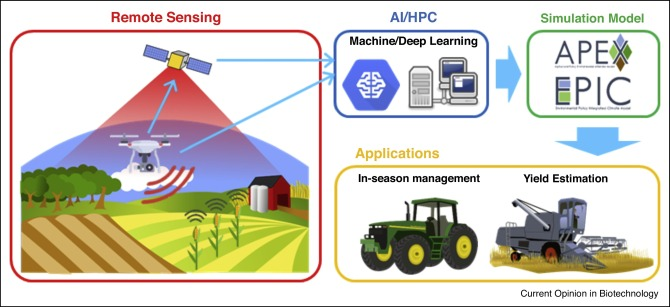
\includegraphics[width=12cm]{1-s2.0-S0958166920301257-gr3.jpg}
     \label{fig:enter-label}
\end{figure}
\section{Methodology}
Automated agricultural monitoring typically involves several key steps: 
\begin{enumerate}
    \item\textbf{ Data Collection:}\hspace{0.2cm}Utilizing various sources such as web camera,sensors, drones and AI devices to gather data on crop, soil levels and other relevant parameters
\item\textbf{ Data Prpcessing:}\hspace{0.2cm}Processing the collected data using techniques like image Processing, machine learning to extract and identity crop growth, infestations and more.
\item\textbf{ Feature Extraction:}\hspace{0.2cm}Identifying relevant features like vegetation indices(NDVI,NDRE),temperature,soil characteristics which are indicative crop health.
\item\textbf{Model Development:}Developing predictive models based on the extracted features to forecast crop yields,predict pest outbreaks and optimize resource allocation(water,fertilizers).
\item\textbf{ Visualization And Decision Support:}Enabling farmers to make informed decisions regarding crop management and risk mitigation.
\item\textbf{ Feedback Loop:}Continuously refining the monitoring system by incorporating feedback from users, updating models with new data, and integrating new technologies to improve accuracy and effectiveness over time.
\end{enumerate}
\section{Argument}
\subsection{Inferiority in Farming}
"Inferiority in farming" refers to the condition where certain farming practices, technologies, or agricultural systems are deemed to be less effective, efficient, or productive compared to alternative methods. This can result from various factors such as outdated techniques, inadequate resources, environmental constraints, or lack of access to modern agricultural inputs and technologies. Inferiority in farming can hinder farmers' ability to optimize their yields, reduce costs, and adapt to changing market demands, ultimately impacting their livelihoods and the sustainability of agricultural production.
\begin{figure}[th]
    \centering
    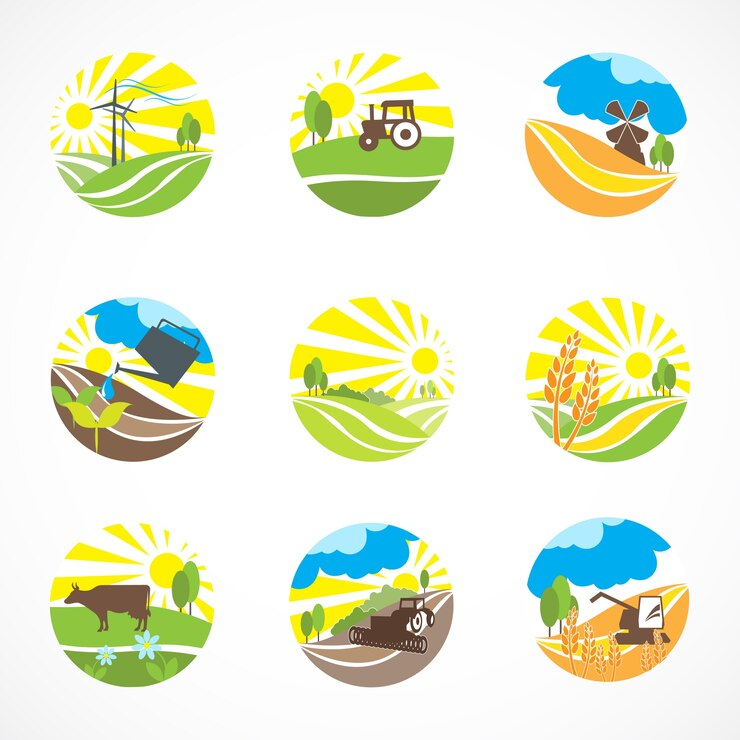
\includegraphics[width=7cm]{nine-farm-scenes_1284-748.jpg}
    \label{fig:enter-label}
\end{figure}
\newpage
\subsection{Agricultural Challenges}
\begin{enumerate}
    \item The first problem is limited access to modern farming technologies and equipment in rural areas.
\item Secondly there is a lack of knowledge and training on sustainable agricultural practices among farmers.
\item Another challenge is the inadequate irrigation infrastructure which affects crop production during dry seasons.
\item Addictionally, high input costs such as fertilizers,seeds and machinery hinder the growth of large scale agriculture.
\item Moreover,climate change and unpredictable weather patterns pose a significant risk to crop yields.
\item The prevalence of pests and diseases that can destroy entire harvests.
\item Furthermore,inadequate transport and storage facilities often result in post havest losses for farmers.
\end{enumerate}



\begin{figure}[th]
    \centering
    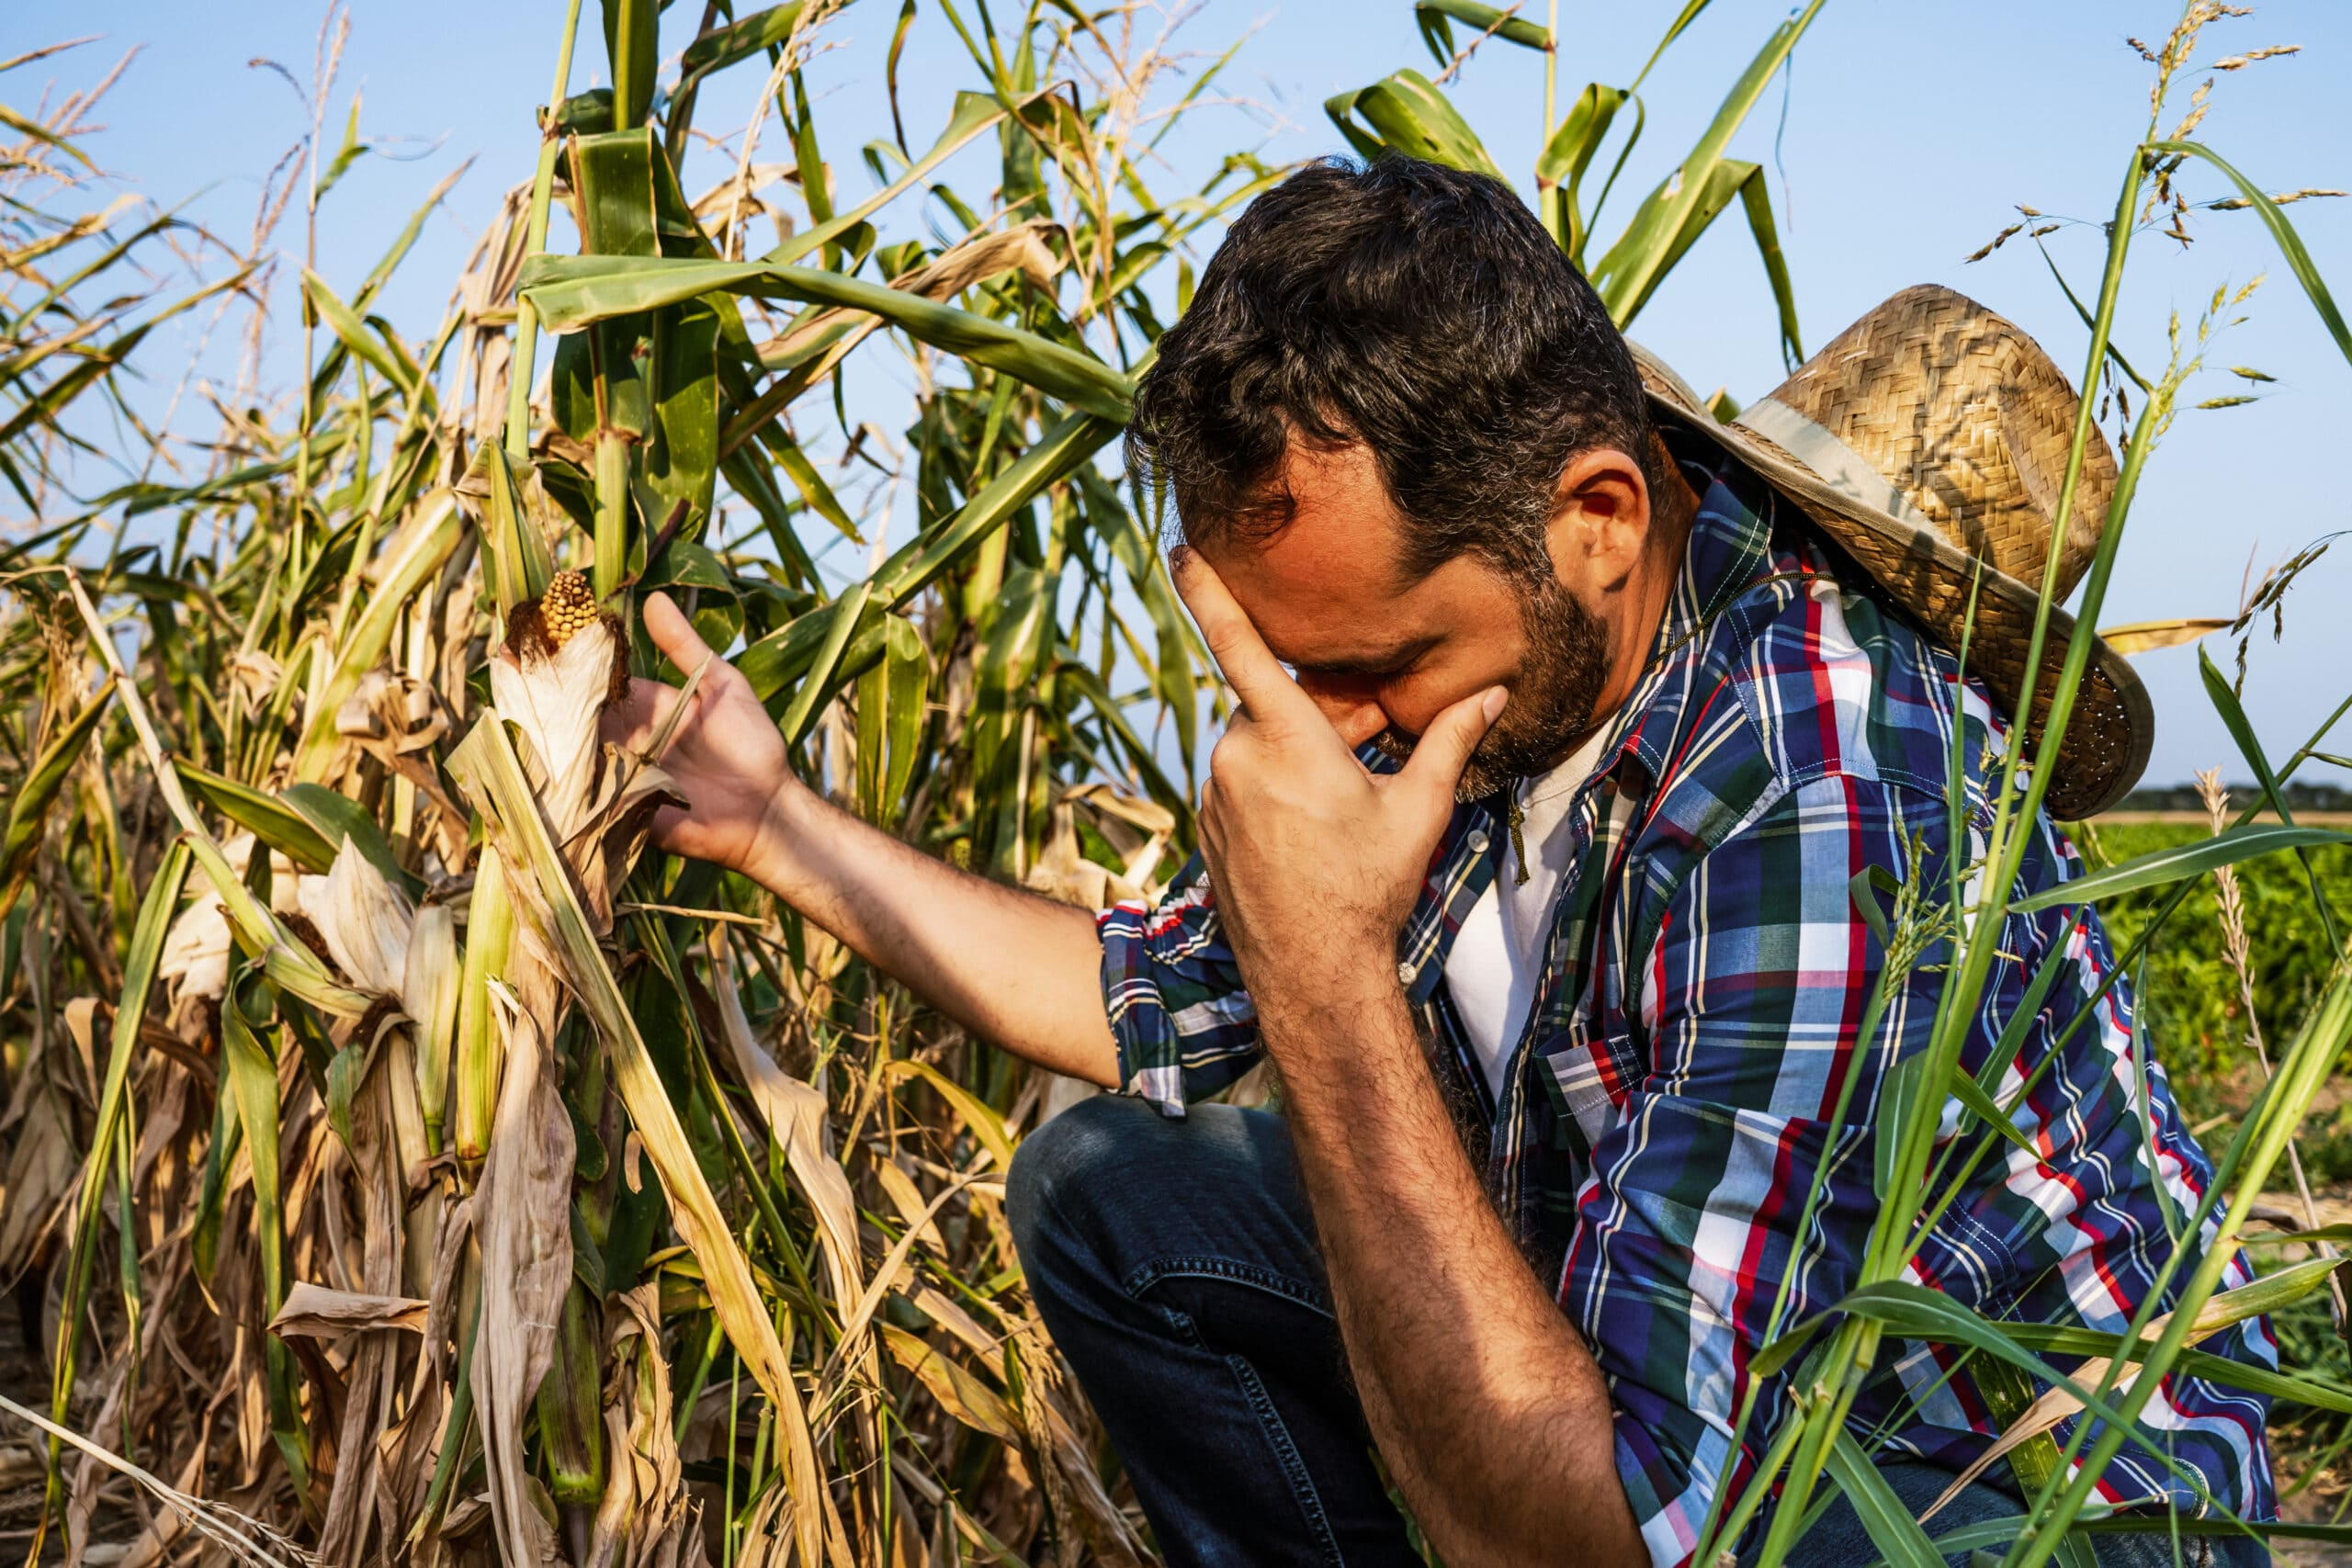
\includegraphics[width=7cm]{received_411749457976133.jpeg}
     \label{fig:enter-label}
\end{figure}
\newpage
\section{Global Vertical Farming Market}
\begin{figure}[th]
    \centering
    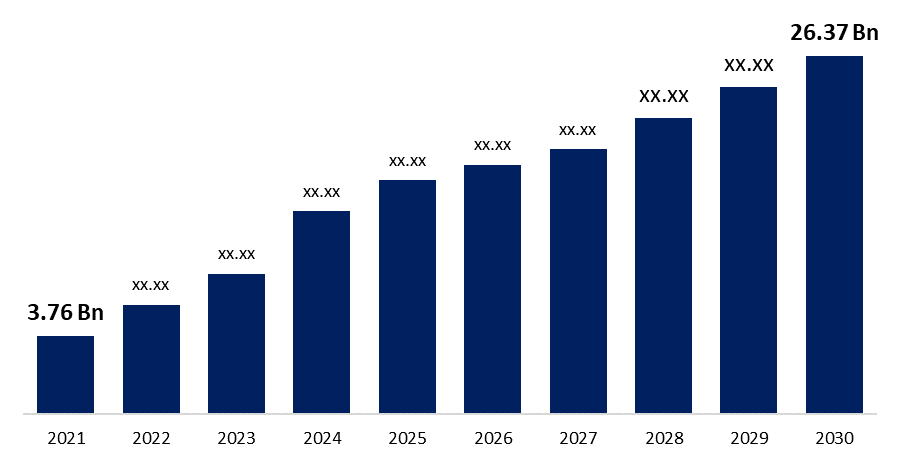
\includegraphics[width=12cm]{vertical-farming-market.png}
    \label{fig:enter-label}
\end{figure}
\section{Benefits}
\begin{enumerate}
    \item\textbf{ Increased crop yields and quality:} Precise irrigation and fertilization lead to healthier crops, higher 
yields, and improved quality.
\item\textbf{Reduced water usage: } By optimizing irrigation, farmers can conserve water, a precious resource facing 
increasing scarcity.
\item\textbf{Reduced fertilizer use and environmental impact: }Targeted fertilization minimizes waste, lowers 
costs, and reduces pollution from excess nutrients.
\item\textbf{Improved soil health:} Monitoring and adjusting practices based on real-time data promotes healthy soil 
ecosystems with good structure and microbial activity.
\item\textbf{Data-driven decision making: } Farmers can base their decisions on objective data analysis instead of 
guesswork, improving overall farm management.
\end{enumerate}
\section{Challenges and Limitations:}
\begin{enumerate}
\item \textbf{Technology Adoption:} Farmers often encounter resistance in adopting new technologies, primarily due to a lack of awareness, insufficient training, or inadequate infrastructure in remote areas.
\item\textbf{Data Security:} The The paramount concern lies in ensuring the security of sensitive farm data. Guarding against unauthorized access, potential data breaches, or misuse of information is of utmost importance.
\item\textbf{ Regulatory Hurdles:} Navigating through existing agricultural and data privacy regulations presents a considerable challenge. Full compliance with diverse regulatory frameworks is imperative for the widespread implementation of automated agricultural monitoring systems.
\item\textbf{Improved soil health:} Monitoring and adjusting practices based on real-time data promotes healthy soil 
ecosystems with good structure and microbial activity.
\item\textbf{Initial Costs:} The upfront investment required for technology adoption poses a significant hurdle, especially for small-scale farmers with limited financial resources.
\newpage
\section{Case Studies or Examples:} A dairy farm in New Zealand employs robotic milking machines that allow cows to be milked at their convenience. This reduces the need for manual labor and increases milk production efficiency.
The Netherlands showcases advancements in automated monitoring with Dutch farms embracing technologies that enhance greenhouse automation and facilitate data-driven decision-making.
A notable case from the U.S. Midwest demonstrates how precision agriculture, incorporating automated monitoring, led to optimized crop yields and resource utilization.
A rice farm in Southeast Asia employs satellite imagery to monitor the growth of rice paddies. When signs of disease or stress are detected, the farmer can quickly respond with targeted interventions, preserving crop quality.
A cotton farm in the United States uses drones to monitor its fields. By analyzing multispectral imagery, the farmer can detect areas with low crop vigor and take corrective actions, such as adjusting irrigation or fertilization.
An Australian wheat farm employs AI algorithms to predict wheat yields based on historical data and current weather conditions. This allows them to adjust planting and harvesting schedules for maximum efficiency.
\begin{figure}[th]
    \centering
    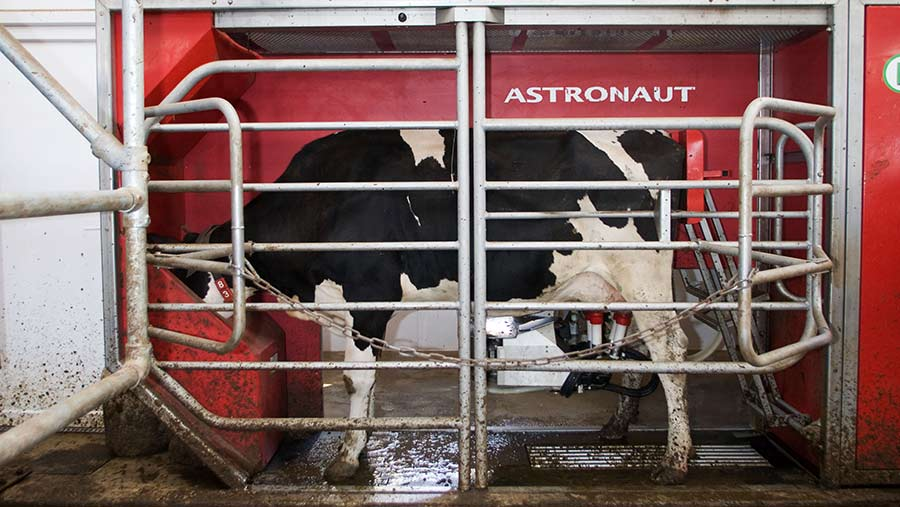
\includegraphics[width=10cm]{1-MAIN-diary-robot-TS-2565-c-Tim-Scrivener.jpg}
     \label{fig:enter-label}
\end{figure}
\section{Comparative Analysis:}
\subsection{Yield Optimization:} 
Automated systems consistently demonstrate their ability to accurately predict optimal irrigation and fertilization, resulting in substantial increases in yields compared to traditional manual methods.
\subsection{Resource Efficiency:}
Automated monitoring exemplifies its prowess in significantly reducing resource wastage by precisely tailoring interventions. This stands in stark contrast to manual, broad-scale approaches that often lack the precision needed for efficient resource utilization.
\section{Economic Impact:}
\subsection{Cost-Benefit Analysis:}
Conducting a meticulous analysis of the expenses related to implementing automated monitoring systems is crucial. This analysis encompasses the initial investment, day-to-day operational costs, and maintenance expenditures. It aims to weigh these costs against the potential returns, including heightened productivity and more efficient resource utilization.
\subsection{Sector-wide Benefits:}
Delving into a comprehensive discussion regarding how the widespread adoption of automated agricultural monitoring can yield substantial economic benefits for the entire agricultural sector. This encompasses the creation of employment opportunities, enhanced global competitiveness, and overall economic growth within the industry.
\section{Conclusion}
In summary, the implementation of automated farming monitoring stands as a pivotal advancement in agriculture, profoundly elevating the intelligence and efficiency of farming practices. Through this report, we have unraveled the positive outcomes stemming from this technology, including amplified crop yields, prudent use of resources, and the overarching economic progression of stakeholders within the farming community. Beyond these immediate benefits, the report concludes with an optimistic outlook, envisioning continual advancements in this field that will shape the future of agriculture.
Furthermore, it is imperative to acknowledge the role of automated agricultural monitoring in aligning with the second goal of the Sustainable Development Goals (SDGs) – Zero Hunger. By providing real-time insights into crop health, optimizing resource usage, and facilitating early detection of issues like pest infestations, this technology becomes a potent tool in ensuring food security. The precision and efficiency it introduces to farming practices contribute significantly to the global effort to eradicate hunger and achieve sustainable agricultural practices. As we advance in this technological era, the prospect of attaining the ambitious goal of Zero Hunger becomes increasingly feasible through the integration of automated farming monitoring systems.
\section{Reference}
\begin{enumerate}


  \item  N. Biswas and A. Aslekar, "Improving Agricultural Productivity: Use of Automation and Robotics," 2022 International Conference on Decision Aid Sciences and Applications (DASA), Chiangrai, Thailand, 2022, pp. 1098-1104, doi: 10.1109/DASA54658.2022.9765207.
    
    \item Z. Dong, H. Wang, Y. Tang, M. Wang and J. Zhao, "Research on Automatic Driving System of Agricultural Machinery Based on Embedded," 2019 IEEE 3rd Information Technology, Networking, Electronic and Automation Control Conference (ITNEC), Chengdu, China, 2019, pp. 1940-1943, doi: 10.1109/ITNEC.2019.8729302
    \item Y. Wang, J. Wang, S. Ma, X. Jiao, H. Wang and W. Pu, "Research on Automatic Auxiliary System of Intelligent Agricultural Machinery," 2023 IEEE 5th International Conference on Power, Intelligent Computing and Systems (ICPICS), Shenyang, China, 2023, pp. 725-729, doi: 10.1109/ICPICS58376.2023.10235523.
 \item D. Khort, A. Kutyrev, I. Smirnov and I. Voronkov, "Automated System for Designing and Management of Agricultural Technologies in Horticulture," 2020 IEEE International Conference on Problems of Infocommunications. Science and Technology (PIC ST), Kharkiv, Ukraine, 2020, pp. 1-6, doi: 10.1109/PICST51311.2020.9468025
\item Z. Zhang, A. Pan, X. Li and Y. Luo, "Large-Model and Generative-Intelligence Agricultural Robot Systems*," 2023 International Annual Conference on Complex Systems and Intelligent Science (CSIS-IAC), Shenzhen, China, 2023, pp. 752-759, doi: 10.1109/CSIS-IAC60628.2023.10363912. 
\end{enumerate}
\end{enumerate}


\end{document}